% =============================================================================
% Part V: The Final Scientific Framework (Chapters 21--23)
% =============================================================================
\chapter{The Final Research Protocol: CF-TP1}\label{ch:cftp1_protocol}

Protocol \textbf{\texttt{CF-TP1 v1.0}} (\emph{CausalFade Target-Population \& Provenance Transport v1.0}, documented in \texttt{experiments/cohort\_029/CF-TP1-v1.0.md} and \texttt{manuscript/article.tex}) represents the mature mathematical culmination of Project CausalFade. Figure~\ref{fig:cftp1_flow} illustrates its end-to-end architecture from exact-rational world synthesis through cryptographic journaling and stratified pair scoring.

\begin{figure}[htbp]
  \centering
  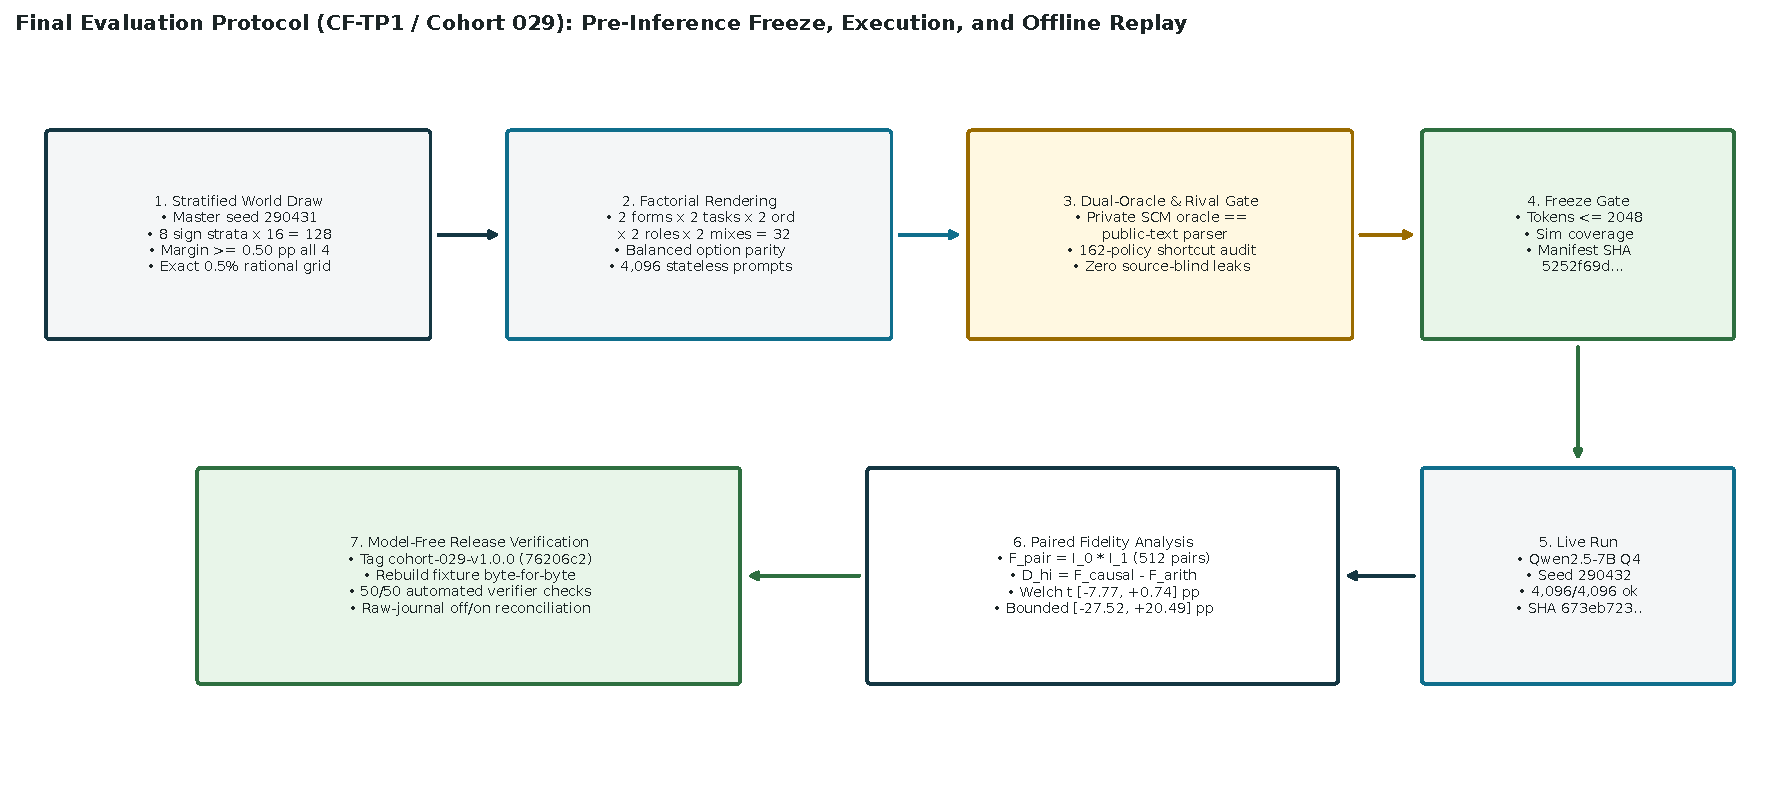
\includegraphics[width=\textwidth]{figures/fig16_cftp1_protocol_flowchart.pdf}
  \caption{End-to-end architecture of the confirmatory \texttt{CF-TP1} benchmark protocol (Cohort~029): exact-rational world quartet synthesis, $162$-policy deterministic shortcut verification, $32$-item per-family factorial expansion, SHA-256 manifest freeze, append-only \texttt{events.jsonl} inference logging, and stratified family-cluster contrast estimation.}
  \label{fig:cftp1_flow}
\end{figure}

% =============================================================================
\section{Exact-Rational World Synthesis and Feasibility Constraints}

Each independent benchmark family $i \in \{0,\dots,127\}$ consists of two displayed study tables---internally indexed as role $r \in \{0,1\}$ (Source~L and Source~R)---over two pre-treatment strata $s \in \{0,1\}$ (\texttt{Amber} and \texttt{Blue}) and binary actions $a \in \{0,1\}$ (\texttt{off} and \texttt{on}), accompanied by two target population Amber shares $w_{i,0} < w_{i,1}$ expressed as exact integer percentages $w_{i,m} \in \{1,\dots,99\}\%$.

\begin{enumerate}
  \item \textbf{Exact Half-Percent Outcome Grid:} Every displayed group-action success rate $\mu_{i,r}(s,a)$ is an integer multiple of $0.5\%$ ($\mu_{i,r}(s,a) = t_{i,r,s,a} / 200$ for integer ticks $t_{i,r,s,a} \in [70, 130]$, i.e., $35.0\%$ to $65.0\%$). Consequently, every printed number in every prompt has \textbf{exact finite one-decimal representation} (\texttt{54.0\%}, \texttt{47.5\%}), eliminating rounding-induced sign discrepancies between internal SCM truth and prompt text!
  \item \textbf{Bi-Directional SCM Realizability (Role-Swap Symmetry):} Crucially, \emph{both} table L and table R are verified by exact rational solver (\texttt{worlds.jsonl} field \texttt{scm}) to be simultaneously realizable as (a) an unconfounded randomized trial over $(\text{Amber}, \text{Blue})$ \emph{and} (b) the marginal stratum rates of a confounded historical study driven by binary unmeasured risk $U \in \{0,1\}$ with valid probabilities in $(0,1)$! Because both tables come from the exact same feasible distribution, \textbf{no numerical property of a table can reveal whether it is the randomized study or the historical study}---eliminating Cohort~016's magnitude shortcut by construction!
  \item \textbf{Four-Corner Target Effect Matrix and Balanced $2\times 2$ Sign Strata:} For each family $i$, let $\Delta_{i}(r, m)$ denote the exact rational standardized effect when table $r \in \{0,1\}$ is the governing randomized source (or designated scorecard) and target Amber weight is $w_{i,m}$ ($m \in \{0,1\}$):
  \begin{equation}
    \Delta_{i}(r, m) = w_{i,m}\bigl(\mu_{i,r}(0,1) - \mu_{i,r}(0,0)\bigr) + (1 - w_{i,m})\bigl(\mu_{i,r}(1,1) - \mu_{i,r}(1,0)\bigr).
    \label{eq:cftp1_corners}
  \end{equation}
  Every corner is bounded strictly away from zero ($|\Delta_i(r,m)| \ge 0.5\pp$), so optimal actions $g_i(r,m) = \mathbb{I}(\Delta_i(r,m) > 0) \in \{0,1\}$ are uniquely defined without ties. Across the $128$ families, rejection sampling (\texttt{seed=290431}) populates $H=8$ balanced strata of $16$ families crossing initial corner sign $b \in \{-1, +1\}$ with two binary switching indicators $(p, g) \in \{0,1\}^2$ ($32$ families per sign-matrix class; Figure~\ref{fig:reversal_retention}A):
  \begin{itemize}
    \item \textbf{Both Stable ($p=0, g=0$, $32$ families):} $g_i(r,0) = g_i(r,1)$ for both roles $r$, and $g_i(0,m) = g_i(1,m)$ for both mixes $m$ (all four corners share one optimal action).
    \item \textbf{Role Switches ($p=0, g=1$, $32$ families):} Changing which source is randomized flips the optimal action ($g_i(0,m) \neq g_i(1,m)$), while changing target mix $w_0 \to w_1$ preserves it ($g_i(r,0) = g_i(r,1)$).
    \item \textbf{Mix Switches ($p=1, g=0$, $32$ families):} Changing target mix $w_0 \to w_1$ flips the optimal action ($g_i(r,0) \neq g_i(r,1)$), while changing source role preserves it ($g_i(0,m) = g_i(1,m)$).
    \item \textbf{Both Switch ($p=1, g=1$, $32$ families):} Changing target mix flips the optimal action \emph{and} changing source role flips the optimal action ($g_i(0,0) = g_i(1,1) \neq g_i(0,1) = g_i(1,0)$, a checkerboard $2\times 2$ sign matrix).
  \end{itemize}
\end{enumerate}

Notice the algebraic elegance of this quartet structure: across all $128$ families, \textbf{exactly half ($64$ families $= 256$ transfer target pairs)} require \textbf{decision reversal} when $w_0 \to w_1$ ($p=1$), and \textbf{exactly half ($64$ families $= 256$ transfer target pairs)} require \textbf{decision invariance} ($p=0$); simultaneously, \textbf{exactly half} require reversal when the randomized role swaps between Study~A and Study~B ($g=1$), and \textbf{half} require invariance ($g=0$)!

% =============================================================================
\section{Complete Worked Derivation: Archived Family \texttt{096} and Test Vectors}

\begin{workedexample}[Exact Step-by-Step Derivation of Archived Family \texttt{096}]
In \texttt{experiments/cohort\_029/freeze/fixture/worlds.jsonl} (index $96$, \texttt{family-096}), the world belongs to stratum $(p=1, g=1, b=-1)$ (\emph{Both Switch}), with half-percent integer table ticks \texttt{[[[102, 108], [106, 95]], [[105, 100], [107, 119]]]} and target Amber shares $(w_0, w_1) = (58\%, 83\%)$:
\begin{enumerate}
  \item \textbf{Convert half-percent ticks to exact percentages and stratum treatment effects:}
    \begin{itemize}
      \item \textbf{Role $r=0$ (Table L):}
        \begin{align*}
          \text{Amber } (s=0): &\quad \text{off } \frac{102}{2} = 51.0\%, \quad \text{on } \frac{108}{2} = 54.0\% \implies \delta_{L}(0) = +3.0\pp = +\frac{3}{100},\\
          \text{Blue } (s=1):  &\quad \text{off } \frac{106}{2} = 53.0\%, \quad \text{on } \frac{95}{2} = 47.5\%  \implies \delta_{L}(1) = -5.5\pp = -\frac{11}{200}.
        \end{align*}
      \item \textbf{Role $r=1$ (Table R):}
        \begin{align*}
          \text{Amber } (s=0): &\quad \text{off } \frac{105}{2} = 52.5\%, \quad \text{on } \frac{100}{2} = 50.0\% \implies \delta_{R}(0) = -2.5\pp = -\frac{1}{40},\\
          \text{Blue } (s=1):  &\quad \text{off } \frac{107}{2} = 53.5\%, \quad \text{on } \frac{119}{2} = 59.5\% \implies \delta_{R}(1) = +6.0\pp = +\frac{3}{50}.
        \end{align*}
    \end{itemize}
  \item \textbf{Standardize to both target population compositions $(w_0 = 58/100, \; w_1 = 83/100)$:}
    \begin{align*}
      \Delta(0, 0) &= \frac{58}{100}\left(+\frac{3}{100}\right) + \frac{42}{100}\left(-\frac{11}{200}\right) = \frac{348 - 462}{20000} = -\frac{57}{10000} = -0.570\pp < 0 \implies g(0,0) = \mathbf{0},\\
      \Delta(0, 1) &= \frac{83}{100}\left(+\frac{3}{100}\right) + \frac{17}{100}\left(-\frac{11}{200}\right) = \frac{498 - 187}{20000} = +\frac{311}{20000} = +1.555\pp > 0 \implies g(0,1) = \mathbf{1},\\
      \Delta(1, 0) &= \frac{58}{100}\left(-\frac{1}{40}\right) + \frac{42}{100}\left(+\frac{3}{50}\right) = \frac{-145 + 252}{10000} = +\frac{107}{10000} = +1.070\pp > 0 \implies g(1,0) = \mathbf{1},\\
      \Delta(1, 1) &= \frac{83}{100}\left(-\frac{1}{40}\right) + \frac{17}{100}\left(+\frac{3}{50}\right) = \frac{-415 + 204}{20000} = -\frac{211}{20000} = -1.055\pp < 0 \implies g(1,1) = \mathbf{0}.
    \end{align*}
    Notice that all four exact fractions (\texttt{-57/10000}, \texttt{311/20000}, \texttt{107/10000}, \texttt{-211/20000}) match \texttt{worlds[96]["corners"]} byte-for-byte!
  \item \textbf{Worked Scoring Test Vectors on Family \texttt{096} ($r=0$, gold pair $(g_0, g_1) = (0, 1)$):}
    \begin{itemize}
      \item \emph{Vector 1 (Causal Oracle, $(\hat{a}_0, \hat{a}_1) = (0, 1)$):} Item accuracy $= (1+1)/2 = 100\%$; pair fidelity $F_{\mathrm{pair}} = 1 \times 1 = \mathbf{1}$ (valid reversal).
      \item \emph{Vector 2 (Constant Activation Policy, $(\hat{a}_0, \hat{a}_1) = (1, 1)$ --- typical Cohort~029 causal output):} Item accuracy $= (0+1)/2 = 50\%$; pair fidelity $F_{\mathrm{pair}} = 0 \times 1 = \mathbf{0}$ (one-correct failure to reverse).
      \item \emph{Vector 3 (Wrong-Way Reversal, $(\hat{a}_0, \hat{a}_1) = (1, 0)$ --- observed $5$ times in Cohort~029 causal):} Item accuracy $= 0\%$; pair fidelity $F_{\mathrm{pair}} = 0 \times 0 = \mathbf{0}$ (neither correct).
      \item \emph{Vector 4 (Noisy Flipper on an Invariant Pair with $(g_0, g_1)=(1,1)$, outputting $(1,0)$ --- observed $45$ times in Cohort~029 arithmetic):} Item accuracy $= 50\%$; pair fidelity $F_{\mathrm{pair}} = 1 \times 0 = \mathbf{0}$ (invariance violation).
    \end{itemize}
\end{enumerate}
\end{workedexample}

% =============================================================================
\section{Factorial Expansion and the 162-Policy Shortcut Audit}

Each of the $128$ world families expands into $2^5 = 32$ stateless prompts ($4{,}096$ total) across five crossed binary factors:
\begin{enumerate}
  \item \textbf{Wording Form ($f \in \{0,1\}$):} Concise structured \texttt{archive} wording ($f=0$) vs.\ natural-prose \texttt{transfer} wording ($f=1$, primary confirmatory split) where study provenance and group-mix transport are explained in plain narrative sentences without mathematical jargon (\texttt{forms.json}).
  \item \textbf{Task Domain ($q \in \{0,1\}$):} \texttt{causal} intervention advising ($q=0$) vs.\ matched \texttt{arithmetic} scorecard evaluation ($q=1$) using the exact same numbers, target weights, and JSON output schema, replacing ``randomized vs.\ historical study'' with ``designated scorecard vs.\ other scorecard.''
  \item \textbf{Display Order ($o \in \{0,1\}$):} Whether Study~A or Study~B is printed first.
  \item \textbf{Role Assignment ($r \in \{0,1\}$):} Which table (L or R) is assigned to the governing randomized study / designated scorecard.
  \item \textbf{Target Population Mix ($m \in \{0,1\}$):} Target Amber share $w_{i,0}$ vs.\ $w_{i,1}$.
\end{enumerate}

Prior to freezing \texttt{manifest.json}, \texttt{policy\_audit.json} evaluated \textbf{$162$ deterministic candidate policies} across all $4{,}096$ items (under both tie-breaking conventions \texttt{0} and \texttt{1}), spanning constant actions, first/last option selection, Study~A/B fixed preference, pooled-study averaging, unweighted group averaging, majority-stratum-only rules, largest-effect/largest-rate heuristics, and $144$ fixed-threshold weight-majority / weight-only rules. Every single noncausal or target-blind shortcut failed on switch pairs ($0\%$ switch fidelity for target-blind rules; $\le 25\%$ overall target-pair fidelity for constant/positional policies), proving mathematically that \textbf{only genuine joint use of governing provenance AND target-mix weighting achieves $100\%$ fidelity}.

% =============================================================================
\chapter{The Final Results}\label{ch:final_results}

Because Cohort~029's raw journal (\texttt{events.jsonl}, SHA-256 \texttt{673eb723...}) achieved $4{,}096/4{,}096$ ($100.0\%$) strict JSON validity with zero missing responses, point-identification bounds collapsed to a single point ($\mathrm{Bounds} = [-3.515625\pp, -3.515625\pp]$). Table~\ref{tab:c29_full_breakdown} synthesizes the complete pairwise and single-item decomposition across all axes of \texttt{CF-TP1}, verified identically by \texttt{manuscript/scripts/extract.py} and our independent audit script.

\begin{table}[htbp]
\centering
\footnotesize
\caption{Complete confirmatory decomposition of Cohort~029 (\texttt{Qwen2.5-7B-Instruct Q4\_K\_M}, $4{,}096$ prompts) across wording forms, task domains, contrast axes, and switch/invariance strata.}\label{tab:c29_full_breakdown}
\begin{tabular}{@{}llllrrrr@{}}
\toprule
\textbf{Form} & \textbf{Task} & \textbf{Pair Axis} & \textbf{Stratum} & \textbf{Pairs} & \textbf{Both (2/2)} & \textbf{One (1/2)} & \textbf{Zero (0/2)} \\
\midrule
Transfer ($f=1$) & Causal ($q=0$)     & Target Mix  & Switch Req.\ ($g_0\neq g_1$) & 256 & \textbf{3} (1.17\%)   & 248 & 5 \\
Transfer ($f=1$) & Causal ($q=0$)     & Target Mix  & Invariant ($g_0=g_1$)        & 256 & \textbf{125} (48.83\%) & 0   & 131 \\
Transfer ($f=1$) & Arithmetic ($q=1$) & Target Mix  & Switch Req.\ ($g_0\neq g_1$) & 256 & \textbf{27} (10.55\%)  & 210 & 19 \\
Transfer ($f=1$) & Arithmetic ($q=1$) & Target Mix  & Invariant ($g_0=g_1$)        & 256 & \textbf{119} (46.48\%) & 45  & 92 \\
\midrule
Transfer ($f=1$) & Causal ($q=0$)     & Source Role & Switch Req.\ ($g_0\neq g_1$) & 256 & \textbf{3} (1.17\%)   & 244 & 9 \\
Transfer ($f=1$) & Causal ($q=0$)     & Source Role & Invariant ($g_0=g_1$)        & 256 & \textbf{121} (47.27\%) & 4   & 131 \\
Transfer ($f=1$) & Arithmetic ($q=1$) & Source Role & Switch Req.\ ($g_0\neq g_1$) & 256 & \textbf{67} (26.17\%)  & 140 & 49 \\
Transfer ($f=1$) & Arithmetic ($q=1$) & Source Role & Invariant ($g_0=g_1$)        & 256 & \textbf{126} (49.22\%) & 66  & 64 \\
\midrule
Archive ($f=0$)  & Causal ($q=0$)     & Target Mix  & All ($256$ sw + $256$ inv)   & 512 & \textbf{128} (25.00\%) & 252 & 132 \\
Archive ($f=0$)  & Arithmetic ($q=1$) & Target Mix  & All ($256$ sw + $256$ inv)   & 512 & \textbf{128} (25.00\%) & 242 & 142 \\
\bottomrule
\end{tabular}
\end{table}

Look closely at the four behavioral signatures revealed in Table~\ref{tab:c29_full_breakdown}:
\begin{enumerate}
  \item \textbf{Why Both Aggregate Target-Pair Fidelities Clustered Near $25\%$:} Any constant policy ($\hat{a}\equiv 1$) gets $0/256$ on switch pairs and $128/256$ on balanced invariant pairs, totaling $128/512 = \mathbf{25.00\%}$! Transfer causal ($128/512$), archive causal ($128/512$), and archive arithmetic ($128/512$) all sat right on that $25.00\%$ constant-policy floor, while transfer arithmetic rose only modestly to $146/512$ ($28.52\%$, $\widehat{\Delta} = -3.52\pp$, Welch $t$ 95\% CI $[-7.77, +0.74]\pp$).
  \item \textbf{Total Insensitivity to Both Target Mix and Causal Provenance Under Causal Framing:} On transfer causal items, \texttt{Qwen2.5-7B Q4\_K\_M} achieved \textbf{$3/256$ ($1.17\%$)} on target-mix switches \emph{and} \textbf{$3/256$ ($1.17\%$)} on source-role switches, while keeping its answer unchanged on $256/256$ ($0$ single-errors!) of target-invariant pairs---because emitting \texttt{\{"activate": 1\}} $97.17\%$ of the time ($995/1{,}024$) automatically never flips!
  \item \textbf{Genuine Partial Provenance and Weight Sensitivity Under Arithmetic Scorecard Framing:} When the exact same mathematical operation was framed as a noncausal ``designated scorecard'' task in natural prose (\texttt{transfer}, $q=1$), the model successfully switched answers across designated scorecards on \textbf{$67/256$ ($26.17\%$)} of role-switch pairs ($22\times$ higher than causal's $3/256$!) and switched across target weights on \textbf{$27/256$ ($10.55\%$)} of target-switch pairs ($9\times$ higher than causal's $3/256$!), while moderating its activation rate to $597/1{,}024$ ($58.30\%$). Yet because mental weighted multiplication remained noisy, it also flipped erroneously on $45/256$ target-invariant pairs and $66/256$ role-invariant pairs, compressing its net target-pair fidelity gain to $+3.52\pp$.
  \item \textbf{Option-Order Diagnostic:} Listing \texttt{\{"activate":1\}} first vs.\ \texttt{\{"activate":0\}} first shifted transfer causal activation only slightly ($502/512 = 98.0\%$ vs.\ $493/512 = 96.3\%$), whereas on transfer arithmetic it shifted activation strongly ($356/512 = 69.5\%$ when \texttt{1} was listed first vs.\ $241/512 = 47.1\%$ when \texttt{0} was listed first, a $+22.46\pp$ first-option pull!).
\end{enumerate}

% =============================================================================
\chapter{The Scientific Contribution}\label{ch:scientific_contribution}

What, ultimately, did Project CausalFade contribute to science? Figure~\ref{fig:contrib_map} organizes CausalFade's verified contributions across four domains while demarcating the strict scope boundaries beyond which no claim is made.

\begin{figure}[htbp]
  \centering
  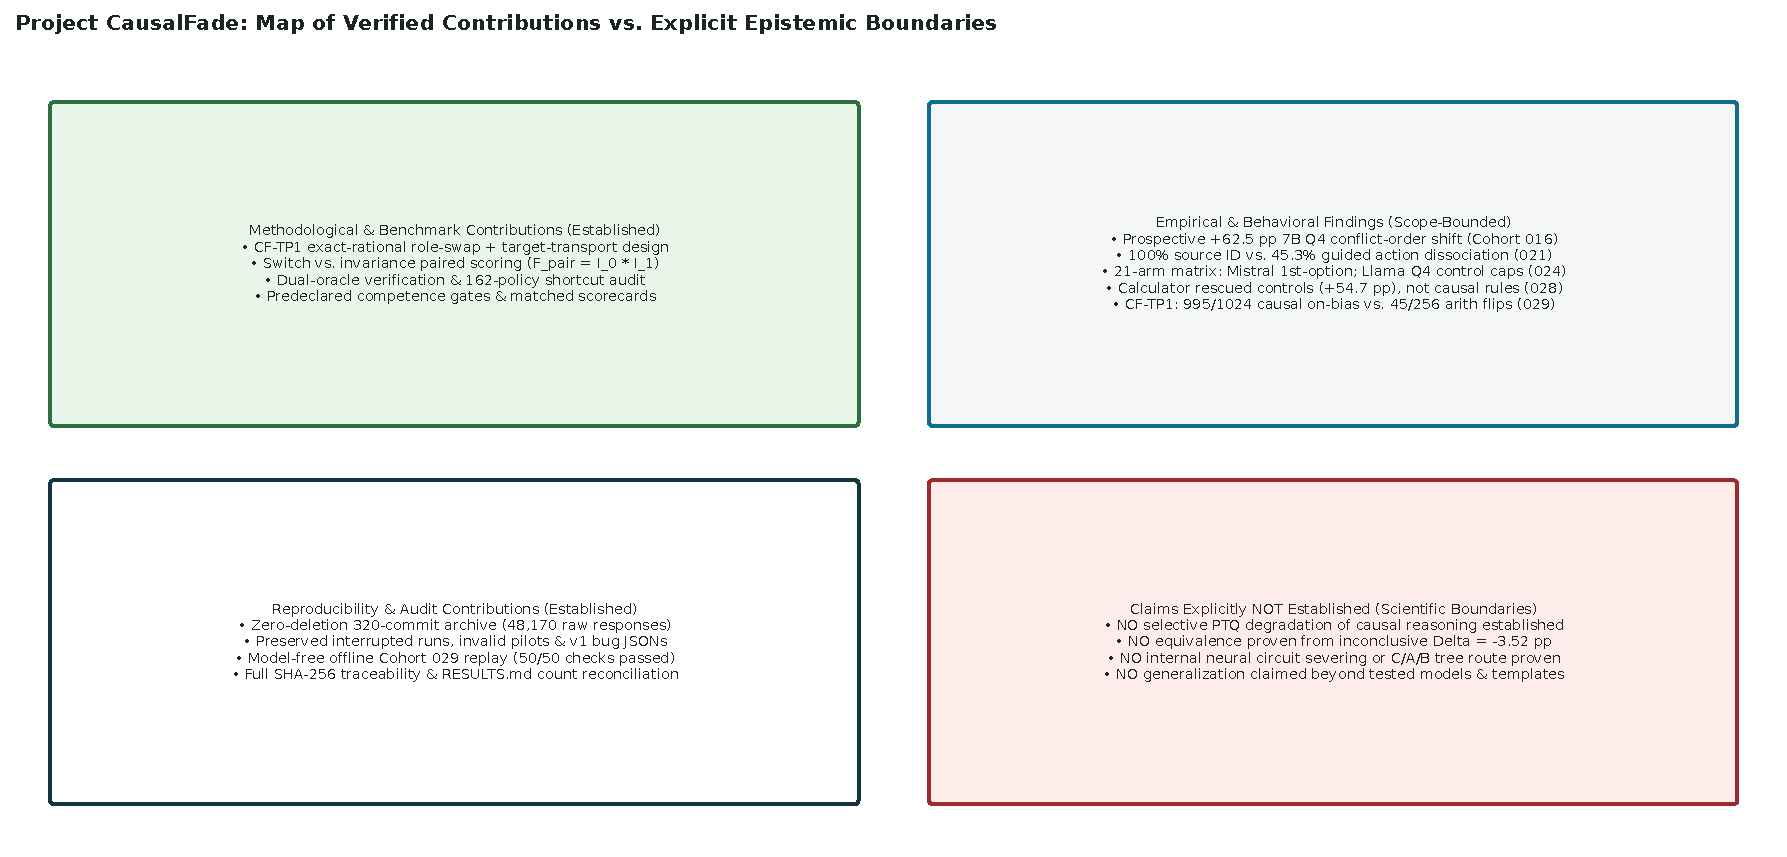
\includegraphics[width=\textwidth]{figures/fig17_research_contribution_map.pdf}
  \caption{Synthesis of CausalFade's lasting scientific contributions across benchmark design, psychometric/diagnostic methodology, LLM failure taxonomy, and reproducibility engineering.}
  \label{fig:contrib_map}
\end{figure}

\section{What CausalFade Established}
\begin{enumerate}
  \item \textbf{The \texttt{CF-TP1} Target-Transport Benchmark Architecture:} An exact-rational, role-symmetric, $162$-policy shortcut-audited benchmark uniting causal provenance selection with subgroup effect transportability and matched noncausal scorecard controls.
  \item \textbf{Pairwise Reversal-and-Retention Decomposition:} Practical demonstration that single-item binary accuracy ($\approx 50\%$) and even aggregate contrast-pair fidelity ($25.0\%$ vs.\ $28.5\%$) conceal radically different underlying policies unless partitioned into required reversals ($3/256$ vs.\ $27/256$) and required invariances ($125/256$ vs.\ $119/256$).
  \item \textbf{Empirical Proof of Three Fundamental Dissociations in Open-Weight Instruction LLMs ($3\text{B}$--$14\text{B}$):}
    \begin{itemize}
      \item \emph{Numeric computation vs.\ explicit action commitment} (Cohorts~002, 006, 007: $95.3\%$--$95.8\%$ ATE sign accuracy vs.\ $0\%$ activation);
      \item \emph{Declarative causal source recognition vs.\ two-source decision integration} (Cohorts~020--022: $100\%$ governing-source ID vs.\ $45.3\%$ guided decisions);
      \item \emph{Tool-assisted arithmetic execution vs.\ structural causal rule selection} (Cohort~028: $+54.69\pp$ Python calculator rescue on noncausal controls vs.\ $+2.34\pp$ on confounder/mediator selection).
    \end{itemize}
  \item \textbf{A Concrete Real-World Shortcut Counterexample (Cohort~016):} Demonstrating on an actual $1{,}536$-response experiment how a $p = 1.24\times 10^{-37}$ prospective replication can coexist with a $100\%$-accurate ($768/768$) source-blind numerical gap shortcut.
\end{enumerate}

\section{What CausalFade Explicitly Did \emph{Not} Establish}
\begin{enumerate}
  \item \textbf{No Selective Quantization Degradation of Causal Reasoning:} Across $48{,}170$ responses, compression never selectively eroded causal reasoning relative to a competent baseline; observed quantization differences reflected 3B arithmetic formula errors (\texttt{Q4\_K\_M}, Cohorts~002/007), 3B 2-bit token looping (\texttt{Q2\_K}, Cohort~001/003), template-specific 7B order sensitivity (Cohort~016), or 8B control-prompt verbosity truncation (\texttt{Llama Q4\_K\_M}, Cohort~024).
  \item \textbf{No Cross-Model or Chain-of-Thought Generalization of Cohort~029:} Cohort~029 evaluated a single open-weight quantized checkpoint (\texttt{Qwen2.5-7B-Instruct Q4\_K\_M}) under stateless single-JSON output without chain-of-thought reasoning tokens or external calculators; how frontier reasoning models or scratchpad-enabled agents perform on \texttt{CF-TP1} remains an open empirical question (Chapter~28).
\end{enumerate}
